\documentclass{article}

\usepackage{pgfplots}
\pgfplotsset{compat=1.16}

\usepackage{microtype}
\usepackage{parskip}

\title{My Report}
\author{Nick}
\date{\today}

\begin{document}

\maketitle

In this report, we study the performance of some algorithms. First, we look at experimental data in Figure 1

\begin{figure}[p]
    \centering
    \begin{tikzpicture}
        \begin{axis}
            \addplot[only marks,mark=x,color=red]table[x=num,y=nick]{data.txt};
            \addplot[only marks,mark=x,color=blue]table[x=num,y=other]{data.txt};
        \end{axis}
    \end{tikzpicture}
    \caption{Experimental performance}
\end{figure}

Now, a look at the theoretical analysis in Figure 2.

\begin{figure}[p]
    \centering
    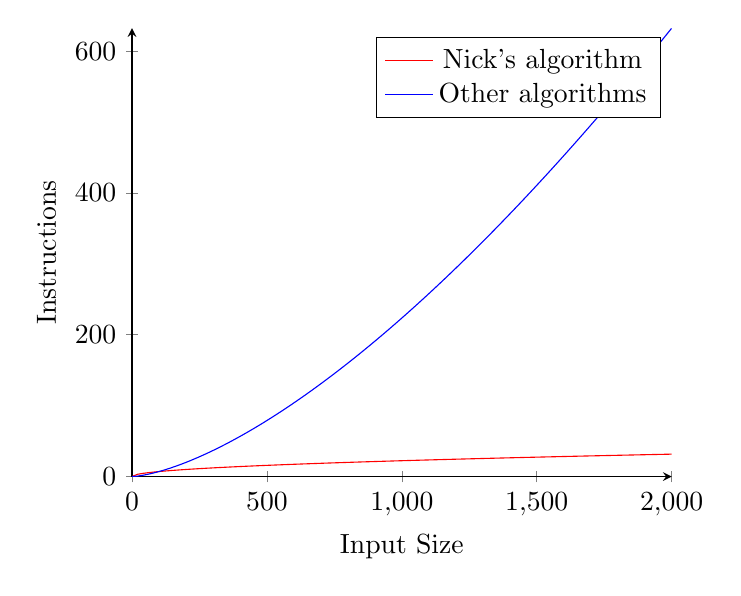
\begin{tikzpicture}
        \begin{axis}[axis lines=left,xlabel={Input Size},ylabel={Instructions}]
            \addplot[domain=0:2000,samples=100,color=red]{sqrt(x/2)};
            \addlegendentry{Nick's algorithm}
            \addplot[domain=0:2000,samples=100,color=blue]{(x/100)*sqrt(x/2)};
            \addlegendentry{Other algorithms}
        \end{axis}
    \end{tikzpicture}
    \caption{Theoretical performance}
\end{figure}

\end{document}